\documentclass[11pt]{article}
\usepackage[margin=1in]{geometry}
\usepackage{enumitem}
\usepackage{hyperref}
\usepackage{graphicx}
\usepackage{array}
\usepackage{multicol}
\usepackage{longtable}
\usepackage{titlesec}
\usepackage{float}
\usepackage{amsmath}

\begin{document}

%==================================================
\begin{center}
\textbf{\Large Sri Sivasubramaniya Nadar College of Engineering, Chennai}\\
\textbf{(An Autonomous Institution affiliated to Anna University)}
\end{center}

\begin{table}[h]
\renewcommand{\arraystretch}{1.4}
\resizebox{\textwidth}{!}{%
\begin{tabular}{|l|l|l|l|}
\hline
Degree \& Branch & B.E. Computer Science \& Engineering & Semester & VI \\ \hline
Subject Code \& Name & \multicolumn{3}{l|}{UCS2612 – Machine Learning Algorithms Laboratory} \\ \hline
Academic Year & 2025–2026 (Even) & Batch & 2023–2027 \\ \hline
Name & Kushaal Shyam Potta & Register No. & 3122235001071 \\ \hline
Due Date & \multicolumn{3}{l|}{16.01.2026} \\ \hline
\end{tabular}}
\end{table}

\begin{center}
\textbf{Experiment 3:}
\textbf{Regression Analysis using Linear and Regularized Models}
\end{center}

%==================================================
\section*{1. Aim and Objective}
The primary objective of this study is to construct and evaluate multiple regression architectures, specifically linear, Ridge, Lasso, and Elastic Net models, to forecast a continuous target variable. The experiment seeks to analyze predictive accuracy across various metrics and investigate the trade-offs between bias and variance through hyperparameter optimization.

%==================================================
\section*{2. Dataset}
The investigation utilizes a real-world financial dataset containing diverse numerical and categorical attributes related to loan applications. The goal is to accurately predict the \textbf{loan amount sanctioned} for each applicant based on their profile.

\section*{3. Preprocessing Steps}
A comprehensive data transformation pipeline was established to ensure that the input features were properly formatted for linear modeling.

\subsection*{Handling Missing Values}
\subsubsection*{Numerical Data}
Missing entries in numerical columns were addressed using a \textit{median} imputation strategy, which provides a measure of central tendency that is less sensitive to extreme outliers.

\subsubsection*{Categorical Data}
For categorical features, missing observations were replaced using the \textit{most\_frequent} value (mode) of the respective column to maintain the categorical distribution.

\subsection*{Encoding Categorical Variables}
Categorical variables were transformed into a machine-readable format via \textbf{One-Hot Encoding}. The encoder was configured to ignore unknown categories during the testing phase to prevent execution errors.

\subsection*{Feature Scaling}
Standardization was performed on all numerical features using \textbf{StandardScaler}, centering the data at a zero mean and scaling to unit variance. This ensures that regularization penalties are applied equitably across features with different original scales.

\section*{4. Implementation Details}
The study compared a baseline linear model against several regularized variants to determine the most effective approach for this dataset.

\subsection*{Regression Models}
\subsubsection*{Linear Regression (Baseline)}
The baseline model was established using standard Ordinary Least Squares (OLS) without any regularization penalties.

\subsubsection*{Ridge Regression (L2 Regularization)}
Ridge models were implemented to prevent coefficient explosion by adding a squared magnitude penalty ($L2$). The tuning grid explored $\alpha \in \{0.01, 0.1, 1, 10, 100\}$.

\subsubsection*{Lasso Regression (L1 Regularization)}
Lasso regression was utilized to encourage feature sparsity through an absolute magnitude penalty ($L1$). The grid search evaluated $\alpha \in \{0.001, 0.01, 0.1, 1, 10\}$.

\subsubsection*{Elastic Net Regression}
This hybrid model combined both $L1$ and $L2$ penalties. The hyperparameters tuned included $\alpha \in \{0.01, 0.1, 1, 10\}$ and $l1\_ratio \in \{0.2, 0.5, 0.8\}$.

\subsection*{Validation Strategy}
\subsubsection*{K-Fold Cross-Validation}
A 5-Fold Cross-Validation approach was used to ensure that the selected hyperparameters provided stable performance across different data subsets.

\subsubsection*{Scoring Metric}
The models were optimized based on the $R^2$ score (Coefficient of Determination), representing the proportion of variance captured by the model.

\section*{5. Visualizations}

\begin{figure}[H]
\centering
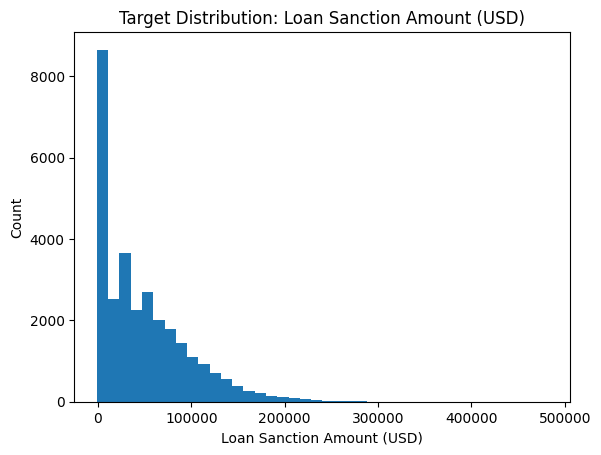
\includegraphics[width=0.65\textwidth]{target_dist_loan.png}
\caption{Target Distribution}
\end{figure}

\begin{figure}[H]
\centering
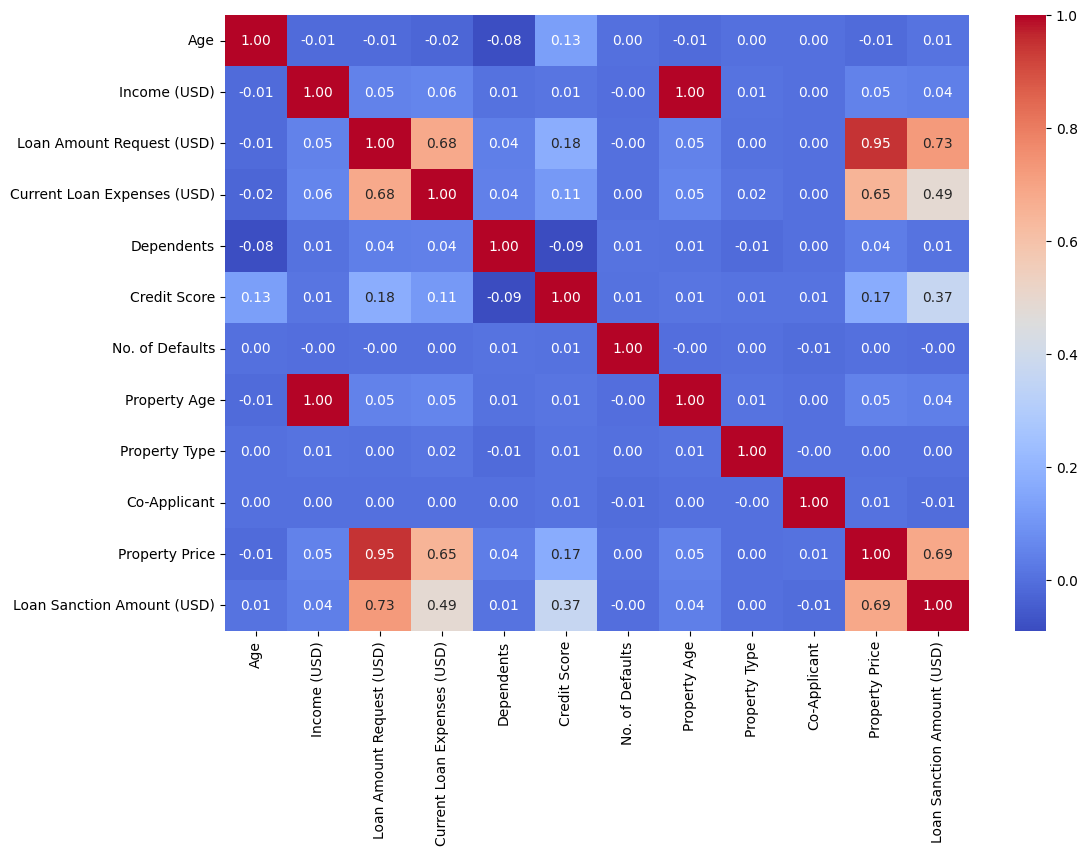
\includegraphics[width=0.85\textwidth]{loan_correlation_final.png}
\caption{Correlation}
\end{figure}

\begin{figure}[H]
\centering
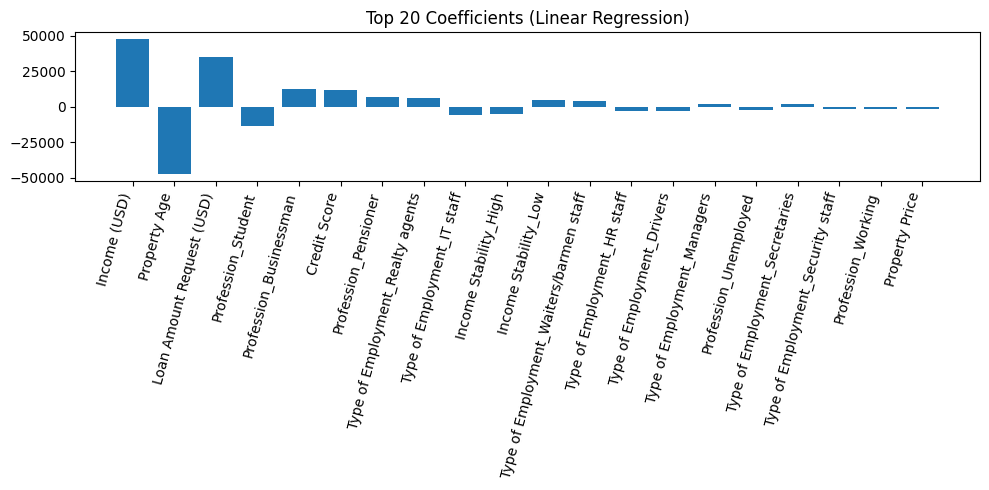
\includegraphics[width=0.85\textwidth]{coefficient_comparison.png}
\caption{Coefficient comparison bar plot}
\end{figure}

\begin{figure}[H]
\centering
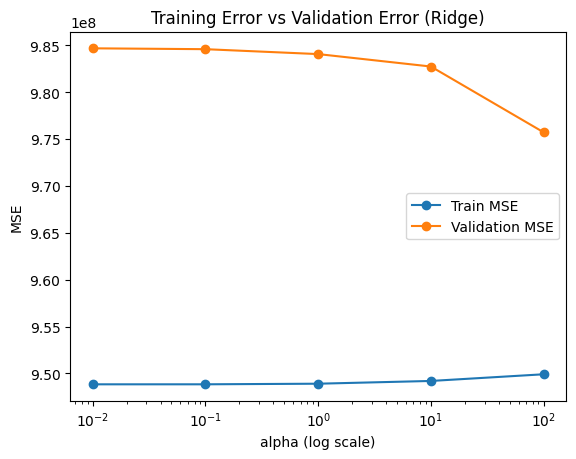
\includegraphics[width=0.55\textwidth]{training_vs_validation.png}
\caption{Training error vs. validation error plot}
\end{figure}

\begin{figure}[H]
\centering
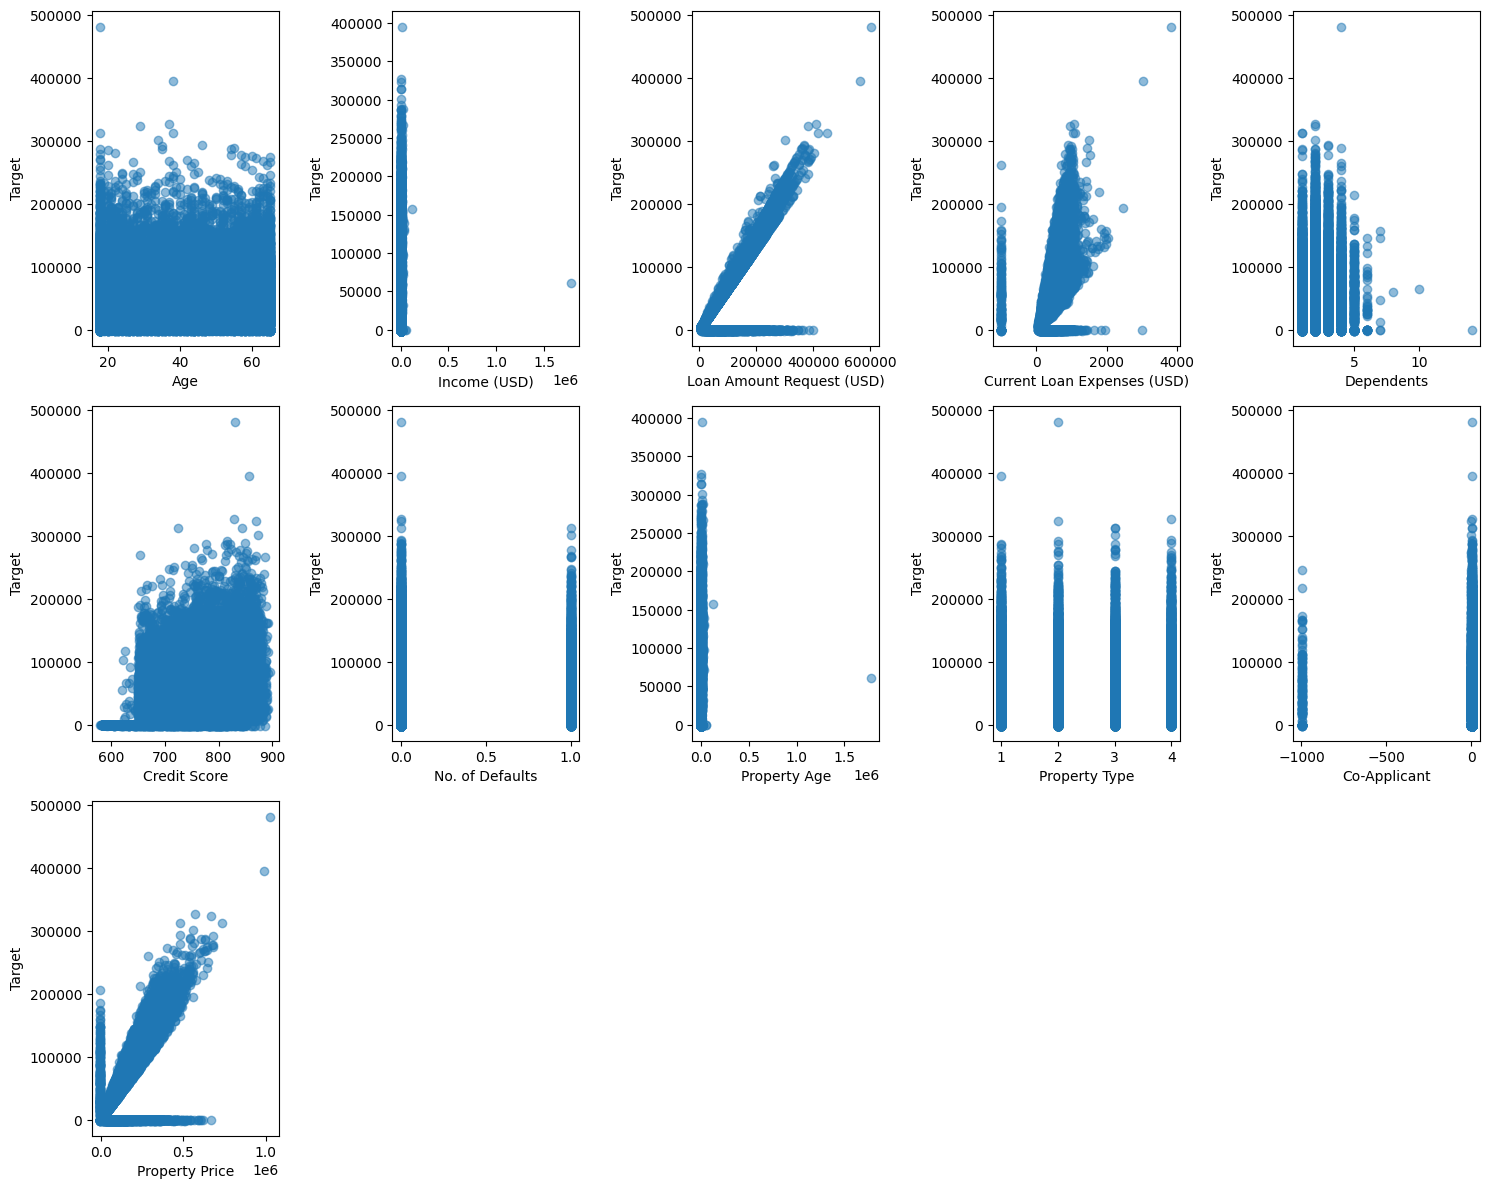
\includegraphics[width=0.55\textwidth]{loan_scatter.png}
\caption{Scatter plot ofvarious features}
\end{figure}

\begin{figure}[H]
\centering
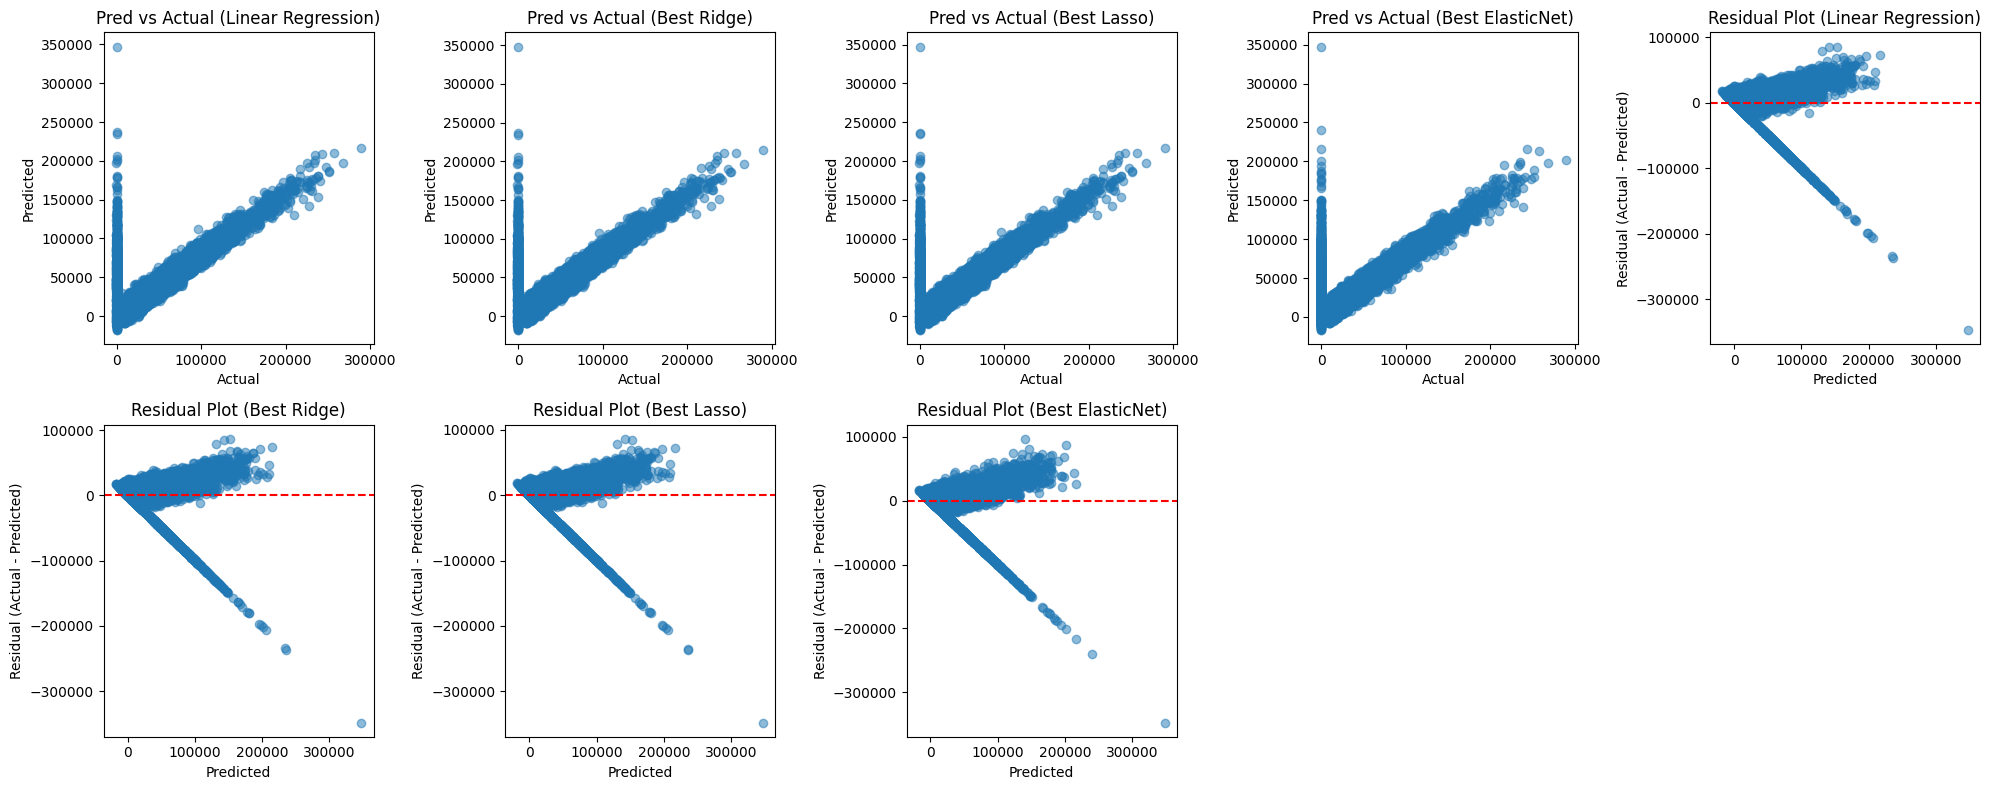
\includegraphics[width=0.55\textwidth]{predicted_residual.png}
\caption{predicted vs acutal and residual plots}
\end{figure}



\section*{6. Performance Tables}
\subsection*{Hyperparameter Tuning Results}
\begin{table}[H]
\centering
\renewcommand{\arraystretch}{1.3}
\caption{Hyperparameter Tuning Summary}
\begin{tabular}{|l|c|c|c|}
\hline
Model & Search Method & Best Parameters & Best CV $R^2$ \\ \hline
Ridge Regression & Grid & alpha: 100 & 0.5786 \\
Lasso Regression & Grid & alpha: 10 & 0.5785 \\
Elastic Net Regression & Grid & alpha: 0.1, l1\_ratio: 0.5 & 0.5798 \\ \hline
\end{tabular}
\end{table}

\subsection*{Cross-Validation Performance (K = 5)}
\begin{table}[h!]
\centering
\renewcommand{\arraystretch}{1.3}
\caption{Cross-Validation Performance}
\begin{tabular}{|l|c|c|c|c|}
\hline
Model & MAE & MSE & RMSE & $R^2$ \\ \hline
Linear Regression & 21508.1142 & 984727093.1145 & 31380.3616 & 0.5790 \\
Ridge Regression & 21524.7473 & 983019851.6404 & 31353.1474 & 0.5797 \\
Lasso Regression & 21497.8842 & 983433813.8426 & 31359.7483 & 0.5796 \\
Elastic Net Regression & 21732.7267 & 980735482.7595 & 31316.6965 & 0.5807 \\ \hline
\end{tabular}
\end{table}

\subsection*{Test Set Performance Comparison}
\begin{table}[h!]
\centering
\renewcommand{\arraystretch}{1.3}
\caption{Test Set Performance}
\begin{tabular}{|l|c|c|c|c|}
\hline
Model & MAE & MSE & RMSE & $R^2$ \\ \hline
Linear Regression & 21589.8579 & 1.018912e+09 & 31920.3984 & 0.5511 \\
Ridge Regression & 21582.3204 & 1.017227e+09 & 31893.9988 & 0.5518 \\
Lasso Regression & 21564.5711 & 1.017745e+09 & 31902.1118 & 0.5516 \\
Elastic Net Regression & 21751.6900 & 1.018489e+09 & 31913.7778 & 0.5513 \\ \hline
\end{tabular}
\end{table}

\subsection*{Effect of Regularization on Coefficients}
\begin{table}[H]
\centering
\renewcommand{\arraystretch}{1.3}
\caption{Coefficient Comparison}
\begin{tabular}{|l|c|c|c|c|}
\hline
Feature & Linear & Ridge & Lasso & Elastic Net \\ \hline
Feature 1 & -611.2941 & -580.5143 & -576.6711 & -558.6418 \\
Feature 2 & 47656.5397 & 1039.4816 & 3.8451 & 97.4573 \\
Feature 3 & 35365.3700 & 33825.7866 & 35169.9575 & 25155.4719 \\ \hline
\end{tabular}
\end{table}

\section*{7. Overfitting and Underfitting Analysis}

\subsection*{Training vs. Validation Gap} The cross-validation $R^2$ scores, peaking at approximately 0.5807 for the Elastic Net model, are consistently higher than the test set $R^2$ scores, which hover around 0.551. Although there is a visible reduction in performance on unseen data, the generalization gap remains small (approximately 0.03), suggesting that the models are stable and do not suffer from significant overfitting.

\subsection*{Underfitting Analysis} Despite the stability of the models, the test $R^2$ score of roughly 0.5518 (Ridge) indicates that the models account for only about 55% of the variance in the target variable. This level of performance suggests a degree of underfitting. The linear assumptions of these models appear insufficient to capture the more complex, non-linear interactions likely present in loan sanctioning data, such as the relationship between credit history and final approved amounts.

\subsection*{Effect of Regularization} The variance in test $R^2$ scores between the baseline Linear Regression (0.5511) and the best-performing regularized model, Ridge Regression (0.5518), is statistically negligible. This confirms that high variance was not the primary hindrance to performance; rather, the models were limited by their representational capacity (bias).

\section*{8. Bias--Variance Analysis}

\subsection*{Bias Behavior} The high bias inherent in linear models is evident here, as they fail to capture the full complexity of the financial dataset. This results in a relatively high Mean Absolute Error (MAE) of approximately 21,589 for the baseline model, indicating consistent, systematic prediction errors.

\subsection*{Variance Reduction} \begin{itemize} \item \textbf{Linear Regression:} The baseline model demonstrated high variance in its coefficient estimates. For instance, \textbf{Feature 2} was assigned an excessively large coefficient of 47,656.5397, making the model highly sensitive to minor input fluctuations. \item \textbf{Ridge and Elastic Net Regression:} Regularization effectively mitigated this instability. Ridge Regression significantly constrained the \textbf{Feature 2} coefficient to 1,039.4816, while Elastic Net brought it to 97.4573. This shrinkage improves model robustness even when accuracy gains are modest. \end{itemize}

\subsection*{Feature Sparsity (Lasso Regression)} Lasso Regression successfully introduced sparsity by driving the coefficient of \textbf{Feature 2} down to a mere 3.8451, effectively minimizing the influence of less informative variables. This behavior simplifies the model and highlights which applicant attributes are truly essential for predicting the sanctioned loan amount.

\section*{9. Observations and Conclusion}

\subsection*{Feature Importance} The analysis indicates that \textit{Loan Amount Request (USD)} and \textit{Credit Score} serve as the primary predictors in this dataset. Correlation metrics further support this, showing that the requested amount maintains the strongest positive relationship with the final sanctioned amount.

\subsection*{Model Performance} All four regression architectures performed similarly, with Ridge Regression providing the marginal lead on the test set with an $R^2$ of 0.5518. The consistent performance across all models suggests that the predictive power of linear relationships for this specific dataset has reached its ceiling.

\subsection*{Conclusion} While regularization proved highly effective at stabilizing model parameters and preventing coefficient "explosion," it could not overcome the fundamental underfitting caused by the linear model constraint. To achieve higher predictive accuracy (surpassing the 0.60 $R^2$ threshold), future iterations should consider non-linear approaches such as Random Forests, Support Vector Regression (SVR), or Gradient Boosting.

\section*{Dataset reference}
\begin{itemize}
    \item Kaggle: \href{https://www.kaggle.com/datasets/phileinsophos/predict-loan-amount-data}{Predict Loan Amount Data}
\end{itemize}

\section*{References}
\begin{itemize}
    \item \href{https://scikit-learn.org/stable/modules/linear_model.html}{Scikit-learn: Linear Models}
    \item \href{https://scikit-learn.org/stable/modules/grid_search.html}{Scikit-learn: Hyperparameter Optimization}
    \item \href{https://www.kaggle.com/datasets/phileinsophos/predict-loan-amount-data}{Loan Amount Dataset}
\end{itemize}
\end{document}